\section{Optymalizator MySQL}

Praktycznie każde zapytanie SQL skierowane do bazy danych MySQL może zostać zrealizowane na wiele różnych sposobów. Optymalizator jest fragmentem oprogramowania serwera MySQL, który odpowiada za wybranie najefektywniejszego sposobu wykonania zapytania (plan wykonania zapytania). 
Proces ten ma kilka etapów. W pierwszym kroku analizator MySQL dzieli zapytanie na tokeny i z nich tworzy "drzewo analizy". Na tym etapie przeprowadzana jest jednocześnie analiza składni zapytania. Następnym etapem jest \textit{preprocessing}, w trakcie którego sprawdzane są między innymi: nazwy kolumn i tabel, a także nazwy i aliasy, aby zapewnić, że nazwy użyte w zapytaniu nie są dwuznaczne. Na kolejnym etapie weryfikowane są uprawnienia. Czynność ta może zajmować szczególnie dużo czasu, jeżeli serwer posiada ogromną liczbę uprawnień. Po zakończeniu etapu \textit{preprocessingu} drzewo analizy jest poprawne i gotowe do tego, aby optymalizator przekształcił je do postaci planu wykonania. 


W MySQL stosowany jest optymalizator kosztowy, co oznacza, że optymalizator szacuje koszt wykonania dla wariantów planu wykonania i wybiera ten z najmniejszym kosztem. Jednostką kosztu jest odczytanie pojedyńczej, losowo wybranej strony danych o wielkości czterech kilobajtów. Wartość kosztu jest wyliczana na podstawie danych statystycznych, dlatego optymalizator wcale nie musi wybrać najbardziej optymalnego planu. Istnieją dwa rodzaje optymalizacji: \textit{statyczna} i \textit{dynamiczna}. Optymalizacja \textit{statyczna} przeprowadzana jest tylko raz i jest niezależna od wartości. To oznacza, że przeprowadzona raz będzie aktualna nawet jeżeli zapytanie będzie wykonywane z różnymi wartościami. Z drugiej strony optymalizacja dynamiczna bazuje na kontekście, w którym wykonywane jest zapytanie i jest przeprowadzana za każdym razem, kiedy polecenie jest wykonywane. Optymalizacja dynamiczna opiera się na wielu parametrach, takich jak: wartości w klauzuli WHERE czy liczba wierszy w indeksie.

Poniżej przedstawione zostało tylko kilka przykładowych typów optymalizacji, które może wykonać moduł optymalizatora.

\begin{itemize}
	\item \textbf{Zmiana kolejności złączeń}. Podczas wykonywania zapytania tabele nie zawsze są złączane w takiej kolejności jak w zapytaniu. Zagadnienie jest dokładniej opisane w podroździale dotyczącym optymalizatora złączeń.
	\item \textbf{Zamiana OUTER JOIN na INNER JOIN.} OUTER JOIN nie zawsze musi być wykonywany jako OUTER JOIN. Niektóre czynniki takie jak warunki w klauzuli WHERE czy schemat bazy danych mogą spowodować, że OUTER JOIN będzie równoznaczne złączeniu INNER JOIN. 
	\item \textbf{Przekształcenia algebraiczne.} Optymzalizator przeprowadza transformacje algebraiczne takie jak: redukcja stałych, eliminowanie nieosiągalnych warunków czy stałych. Przykładowo warunek (2=2 AND a>2) może zostać przekształcony do postaci (a>2. Podobnie warunek (a<b AND b=c AND a=5) może być przekształcony do (b>5 AND b=c AND a=5).
	\item \textbf{Optymalizacja funkcji MIN(), MAX().}
	Serwer już na etapie optymalizacji zapytania może uznać wartości zwracane przez funkcje jako stałe dla reszty zapytania. W niektórych przypadkach optymalizator może nawet pominąć tabelę w planie wykonania zapytania, jeżeli jedyną wartością pobieraną z tabeli jest wynik funkcji MIN() lub MAX(). W takim przypadku w danych wyjściowych polecenia EXPLAIN znajdzie się ciąg tekstowy "Select tables optimized away".
	Na poniższym przykładzie widzimy, że kolumna \textit{ref} dla pierwszego wiersza jest wartość ''const'', czyli najmniejsza wartość id z tabeli Users została potraktowana jako stała.
	\begin{spverbatim}
		EXPLAIN SELECT * FROM Comments WHERE UserId = (SELECT MIN(id) FROM Users);
	\end{spverbatim}
	\begin{figure}[H]
		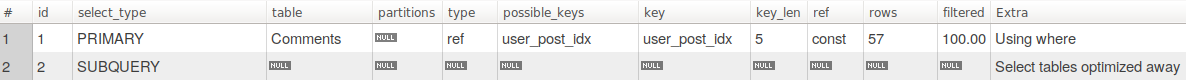
\includegraphics[scale =0.4]{explain20.png} 
	\end{figure}
	\item \textbf{Optymalizacja funkcji COUNT().} Wynik funkcji COUNT(*) bez klauzuli WHERE w niektórych silnikach (np. MyISM), również mogą zostać potraktowane jako stała, ale nie dotyczy to najpopularniejszego obecnie w MySQL silnika InnoDB.
	\textbf{Optymalizacja stałej tabeli}
	
	\item \textbf{Stałe tabele.} \textit{Stała tabela} jest to tabela, która zawiera co najwyżej jeden wiersz lub warunek zawarty w klauzuli WHERE odnosi się do wszystkich kolumn klucza głównego, albo do indeksu UNIQUE NOT NULL. W takim przypadku MySQL może zwrócić wartość jeszcze przed wykonaniem zapytania i potraktować jako stałą dla dalszej części zapytania.
\end{itemize}
////todo opisać więcej przykładów?

\subsection{Dane statystyczne dla optymalizatora}
Przechowywaniem danych statystycznych jest zadaniem silników bazy danych. Z tego powodu w zależności od użytego silnika przechowywane wartości statystyczne mogą być różne. Przykładowo silnik MyISM przechowuje informację o aktualnej liczbie rekordów w tabeli, silnik InnoDB takiej informacji nie przechowuje, natomiast niektóre silniki, np. Archive, w ogólnie nie przechowują danych statystycznych.

\subsection{Plan wykonania zapytania}
Wynikiem optymalizacji jest plan wykonania zapytania. Plan wykonania jest zapisywany w postaci drzewa instrukcji, które kolejno wykonywane doprowadzą do zwrócenia wyniku zapytania.
\begin{spverbatim}
	SELECT * FROM Posts p LEFT JOIN PostTypes pt ON p.PostTypeId = pt.Id LEFT JOIN PostLinks pl ON p.Id = pl.PostId LEFT JOIN LinkTypes lt on pl.LinkTypeId = lt.id WHERE PostID = 9;
\end{spverbatim}
Gdybyśmy mieli wyobrazić sobie sposób łączenia tabel w MySQL zapewne wyobrazilibyśmy sobie to tak, jak na poniższym schemacie.
 \begin{center}
 	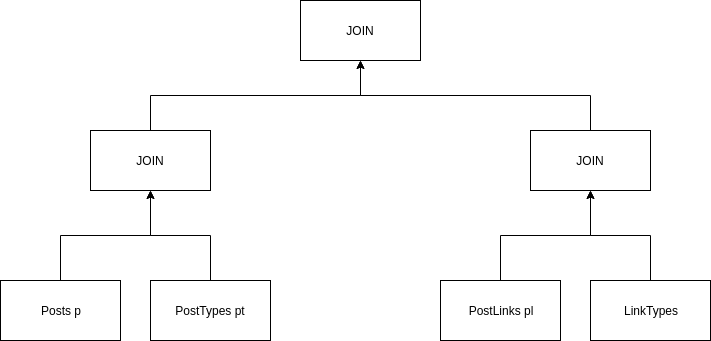
\includegraphics[scale =0.45]{PLAN_WYKONANIA_1.png} 
 \end{center}
W praktyce drzewo instrukcji przybiera postać \textit{drzewa lewostronnie zagnieżdżonego}, co pokazano na rysunku poniżej.
\begin{center}
	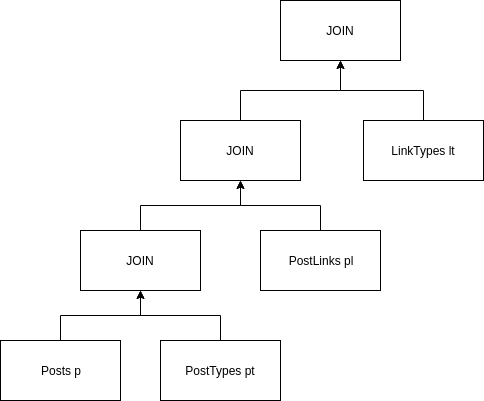
\includegraphics[scale =0.45]{PLAN_WYKONANIA_2.png} 
\end{center}
Wywołując polecenie EXPLAIN dla naszego zapytania, używając klienta MySQL Workbench możemy wyświetlić graficzną postać odpowiadającą drzewu instrukcji.
\begin{center}
	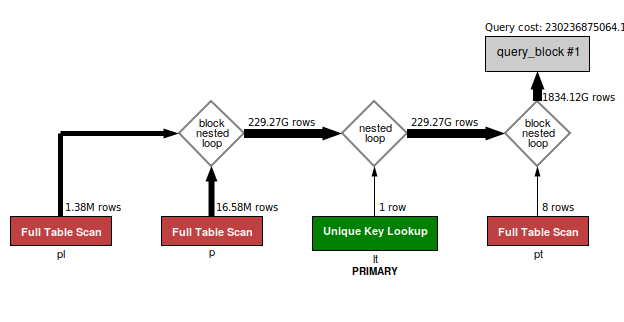
\includegraphics[scale =0.5]{explain21.png} 
\end{center}
Widzimy, że drzewo otrzymane jako wynik polecenia EXPLAIN jest drzewem lewostronnie zagnieżdżonym. Widzimy też, że optymalizator zdecydował się zamienić kolejność złączeń aby zminimalizować koszt wykonania zapytania.

\subsection{Optymalizator złączeń}
Większość operacji złączeń można wykonać na wiele różnych sposobów uzyskując ten sam wynik. Zamiana kolejności jest bardzo skuteczną formą optymalizacji zapytań. Rozważmy teraz następujące przykładowe zapytanie:

\begin{spverbatim}
	SELECT u.Id, p.Id, c.Id, pt.`Type` FROM Users u INNER JOIN Posts p ON u.Id = p.OwnerUserId	INNER JOIN Comments c ON c.UserId = u.Id INNER JOIN PostTypes pt ON pt.Id = p.PostTypeId WHERE u.Id = 4;
\end{spverbatim}

Wywołując polecenie z prefiksem EXPLAIN otrzymujemy następujący wynik:
\begin{center}
	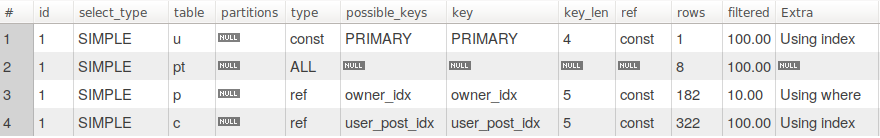
\includegraphics[scale =0.45]{explain22.png} 
\end{center}
Następnie modyfikujemy zapytanie dodając słowo kluczowe STRAIGHT\textunderscore JOIN, aby wymusić kolejność złączeń taką jak w zapytaniu.
\begin{center}
	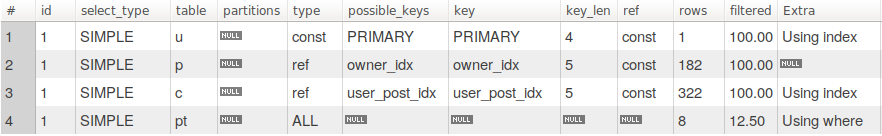
\includegraphics[scale =0.45]{explain23.png} 
\end{center}
Widzimy, że oba rezultaty polecenia są niemalże identyczne, jedyną różnicą jest kolejność dokonywanych złączeń. Sprawdźmy teraz, jaki jest koszt wykonania obu zapytań. Koszt pierwszego zapytania, którego kolejność została zamieniona na etapie optymalizacji wynosi 6510. Koszt drugiego zapytania wynosi 66868! Zamiana kolejności złączeń zmniejszyła koszt dziesięciokrotnie.
W kolejnym kroku włączyłem profilowanie zapytań za pomocą komendy:
\begin{spverbatim}
	SET PROFILING = 1;
\end{spverbatim}, wykonałem 10 zapytań dla każdego wariantu i policzyłem średni czas, jaki serwer MySQL spędzał na etapie ''executing'', czyli etapie faktycznego wykonywania zapytania. Dla zapytania z kolejnością wybraną przez optymalizator otrzymałem wartość 0.04 sekundy, natomiast przy kolejności wybranej przez nas w zapytaniu wartosć ta wynosiła już 0.28 sekundy. Powyższy eksperyment pokazuje, że zamiana kolejności złączeń jest niezwykle wyjadną formą optymalizacji zapytań i może prowadzić do wielokrotnego zmniejszenia kosztu zapytania. Oczywiście nadal może się zdarzyć sytuacja, kiedy zapytanie z wymuszoną kolejnością załączeń będzie wydajniejsze, ponieważ optymalizator MySQL nie zawsze może sprawdzić wszystkie potencjalne kombinacje złączeń, ale w zdecydowanej większości przypadków optymalizator złączeń wygrywa z człowiekiem.

\subsection{Konfiguracja optymalizatora złączeń}
Optymalizator złączeń stara się wygenerować plan zapytań o najniższym możliwym koszcie. W idealnym przypadku optymalizator może zweryfikować wszystkie potencjalne kombinacje złaczeń. Niestety operacja złączeń dla \textit{n} tabel będzie miała \textit{n!} możliwych kombinacji. Oznacza to, że dla dziesięciu tabel złaczenia mogą zostać przeprowadzone na 3628800 różnych sposobów i gdyby optymalizator zdecydował się przetestować każdy dostępny scenariusz, kompilacja mogłaby zająć wiele godzin, a nawet dni. Do zdefiniowania, jak wiele planów powinien przetestować optymalizator służy opcja \textit{optimizer\textunderscore search\textunderscore depth}. Generalnie im niższa wartość zmiennej, tym szybciej optymalizator zwróci plan wykonania, ale zmniejsza się też prawdopodobieństwo optymalności zwróconego planu. Wartość 0 oznacza, że MySQL dla każdego zapytania dobierze odpowiednią (zdaniem optymalizatora) przestrzeń przeszukiwania.

Aby pokazać wpływ parametru \textit{optimizer\textunderscore search\textunderscore depth} przygotowałem następujący kod sql, który tworzy dwie tabele, a następnie wypełnia jest losowymi danymi.

\begin{spverbatim}
	CREATE TABLE `lecturers`
	(
	`id` INT(11) NOT NULL AUTO_INCREMENT,
	PRIMARY KEY (`id`)
	);
	CREATE TABLE `students`
	(
	`id` INT(11) NOT NULL AUTO_INCREMENT,
	`lecturer_id` INT(11) NOT NULL,
	`value` SMALLINT(6) NOT NULL,
	PRIMARY KEY (`id`),
	INDEX `lecturer_id` (`lecturer_id`),
	INDEX `value` (`value`)
	);
	INSERT INTO `lecturers` VALUES (1), (2);
	
	delimiter ;;
	CREATE PROCEDURE fill_tables()
	BEGIN
	DECLARE i int DEFAULT 0;
	WHILE i <= 1000 DO
	INSERT INTO `students` (`id`, `lecturer_id`, `value`) VALUES (0, 1, i);
	INSERT INTO `students` (`id`, `lecturer_id`, `value`) VALUES (0, 2, i);
	SET i = i + 1;
	END WHILE;
	END;;
	delimiter ;
	
	CALL fill_tables();
\end{spverbatim}

Następnie wykonałem wielokrotnie następujące zapytanie 
\begin{spverbatim}
	SELECT COUNT(*) FROM table_parent AS p WHERE 1
	AND EXISTS (SELECT 1 FROM students AS s WHERE s.lecturer_id = p.id AND s.value = 1 LIMIT 1)
	AND EXISTS (SELECT 1 FROM students AS s WHERE s.lecturer_id = p.id AND s.value = 2 LIMIT 1)
	AND EXISTS (SELECT 1 FROM students AS s WHERE s.lecturer_id = p.id AND s.value = 3 LIMIT 1)
	AND EXISTS (SELECT 1 FROM students AS s WHERE s.lecturer_id = p.id AND s.value = 4 LIMIT 1)
	AND EXISTS (SELECT 1 FROM students AS s WHERE s.lecturer_id = p.id AND s.value = 5 LIMIT 1)
	AND EXISTS (SELECT 1 FROM students AS s WHERE s.lecturer_id = p.id AND s.value = 6 LIMIT 1)
	AND EXISTS (SELECT 1 FROM students AS s WHERE s.lecturer_id = p.id AND s.value = 7 LIMIT 1)
	AND EXISTS (SELECT 1 FROM students AS s WHERE s.lecturer_id = p.id AND s.value = 8 LIMIT 1)
	AND EXISTS (SELECT 1 FROM students AS s WHERE s.lecturer_id = p.id AND s.value = 9 LIMIT 1)
	AND EXISTS (SELECT 1 FROM students AS s WHERE s.lecturer_id = p.id AND s.value = 10 LIMIT 1)
\end{spverbatim}
zmieniając parametr \textit{optimizer\textunderscore search\textunderscore depth}, dla każdej wartości zmiennej zapisałem średni czas wykonania polecenia EXPLAIN. Wyniki umieściłem w poniższej tabeli.

\begin{center}
	\begin{tabular}{ |c|c| } 
		\hline
		optimizer\textunderscore search\textunderscore depth & czas [sekund]\\ 
		\hline
		0 & 22\\
		1 & 0.0011\\
		2 & 0.0019\\
		3 & 0.0059\\
		5 & 0.6\\
		10 & 15\\
		20 & 22\\
		30 & 27\\
		62 & 36\\
		\hline
	\end{tabular}
\end{center}
Widzimy, że wraz ze wzrostem wartości parametru wzrastał czas wykonywania zapytania. Kolejnym krokiem było włączenie profilowania i sprawdzenie, na który z etapów serwer spędził najwięcej czasu. Wyniki zostały posortowane według czasu i na poniższym zrzucie ekranu widzimy profil zapytania dla wartości 62.
\begin{center}
	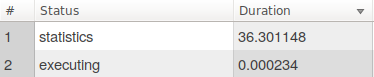
\includegraphics[scale =0.60]{profile1.png} 
\end{center}
Profilowanie zapytania wskazuje nam, że przez praktycznie cały czas serwer starał się zebrać dane, które pozwolą mu wybrać najoptymalniejszy plan wykonania zapytania. Eksperyment wyraźnie pokazuje, że dla pewnych zapytań, próba wybrania najoptymalniejszego rozwiązania może skończyć się gigantycznym wydłużeniem czasu zapytania. Co ciekawe nawet dla wartości 0 optymalizacja okazał się nieefektywna, co prowadzi do wniosku, że czasami jedym rozwiązaniem w przypadku, kiedy serwer zbyt dużą ilość czasu spędza na doborze planu, jest ręczna zmiana wartości parametru optimizer\textunderscore search\textunderscore depth.

OPISAĆ 2 PARAMETR !!!

\subsection{Konfiguracja statystyk tabel InnoDB dla optymalizatora}